\chapter{Introduction to LSTM}

\section{Lesson Overview}
\href{https://www.youtube.com/watch?v=CH9O_fNGR2Q&ab_channel=Udacity}{Youtube} \newline

In this lesson, we will cover the following topics:

\begin{itemize}
    \item LSTM Overview
    \item LSTM Architecture and Gates
\end{itemize}
By the end of the lesson, you'll be able to:

\begin{itemize}
    \item Explain how LSTMs overcome the limitations of RNNs
    \item Implement the LSTM architecture
\end{itemize}

\section{RNN vs LSTM}
\href{https://www.youtube.com/watch?v=70MgF-IwAr8&ab_channel=Udacity}{Youtube}
\subsection{Vanishing Gradient Problem}
The problem with RNNs is that memory stored in an RNN can be effective short-term memory. This is due to the "Vanishing Gradient Problem." The Vanishing Gradient Problem happens when the gradient of a deep layer of the neural network is "diluted" and has a reduced effect on the network. This is due to the nature of the activation functions of the RNN that can diminish the effect of the gradients of the deeper layer over time. \newline

The LSTM solves the problem by introducing an operation to maintain the long-term memory of the network. We will learn about these gates in subsequent lessons.

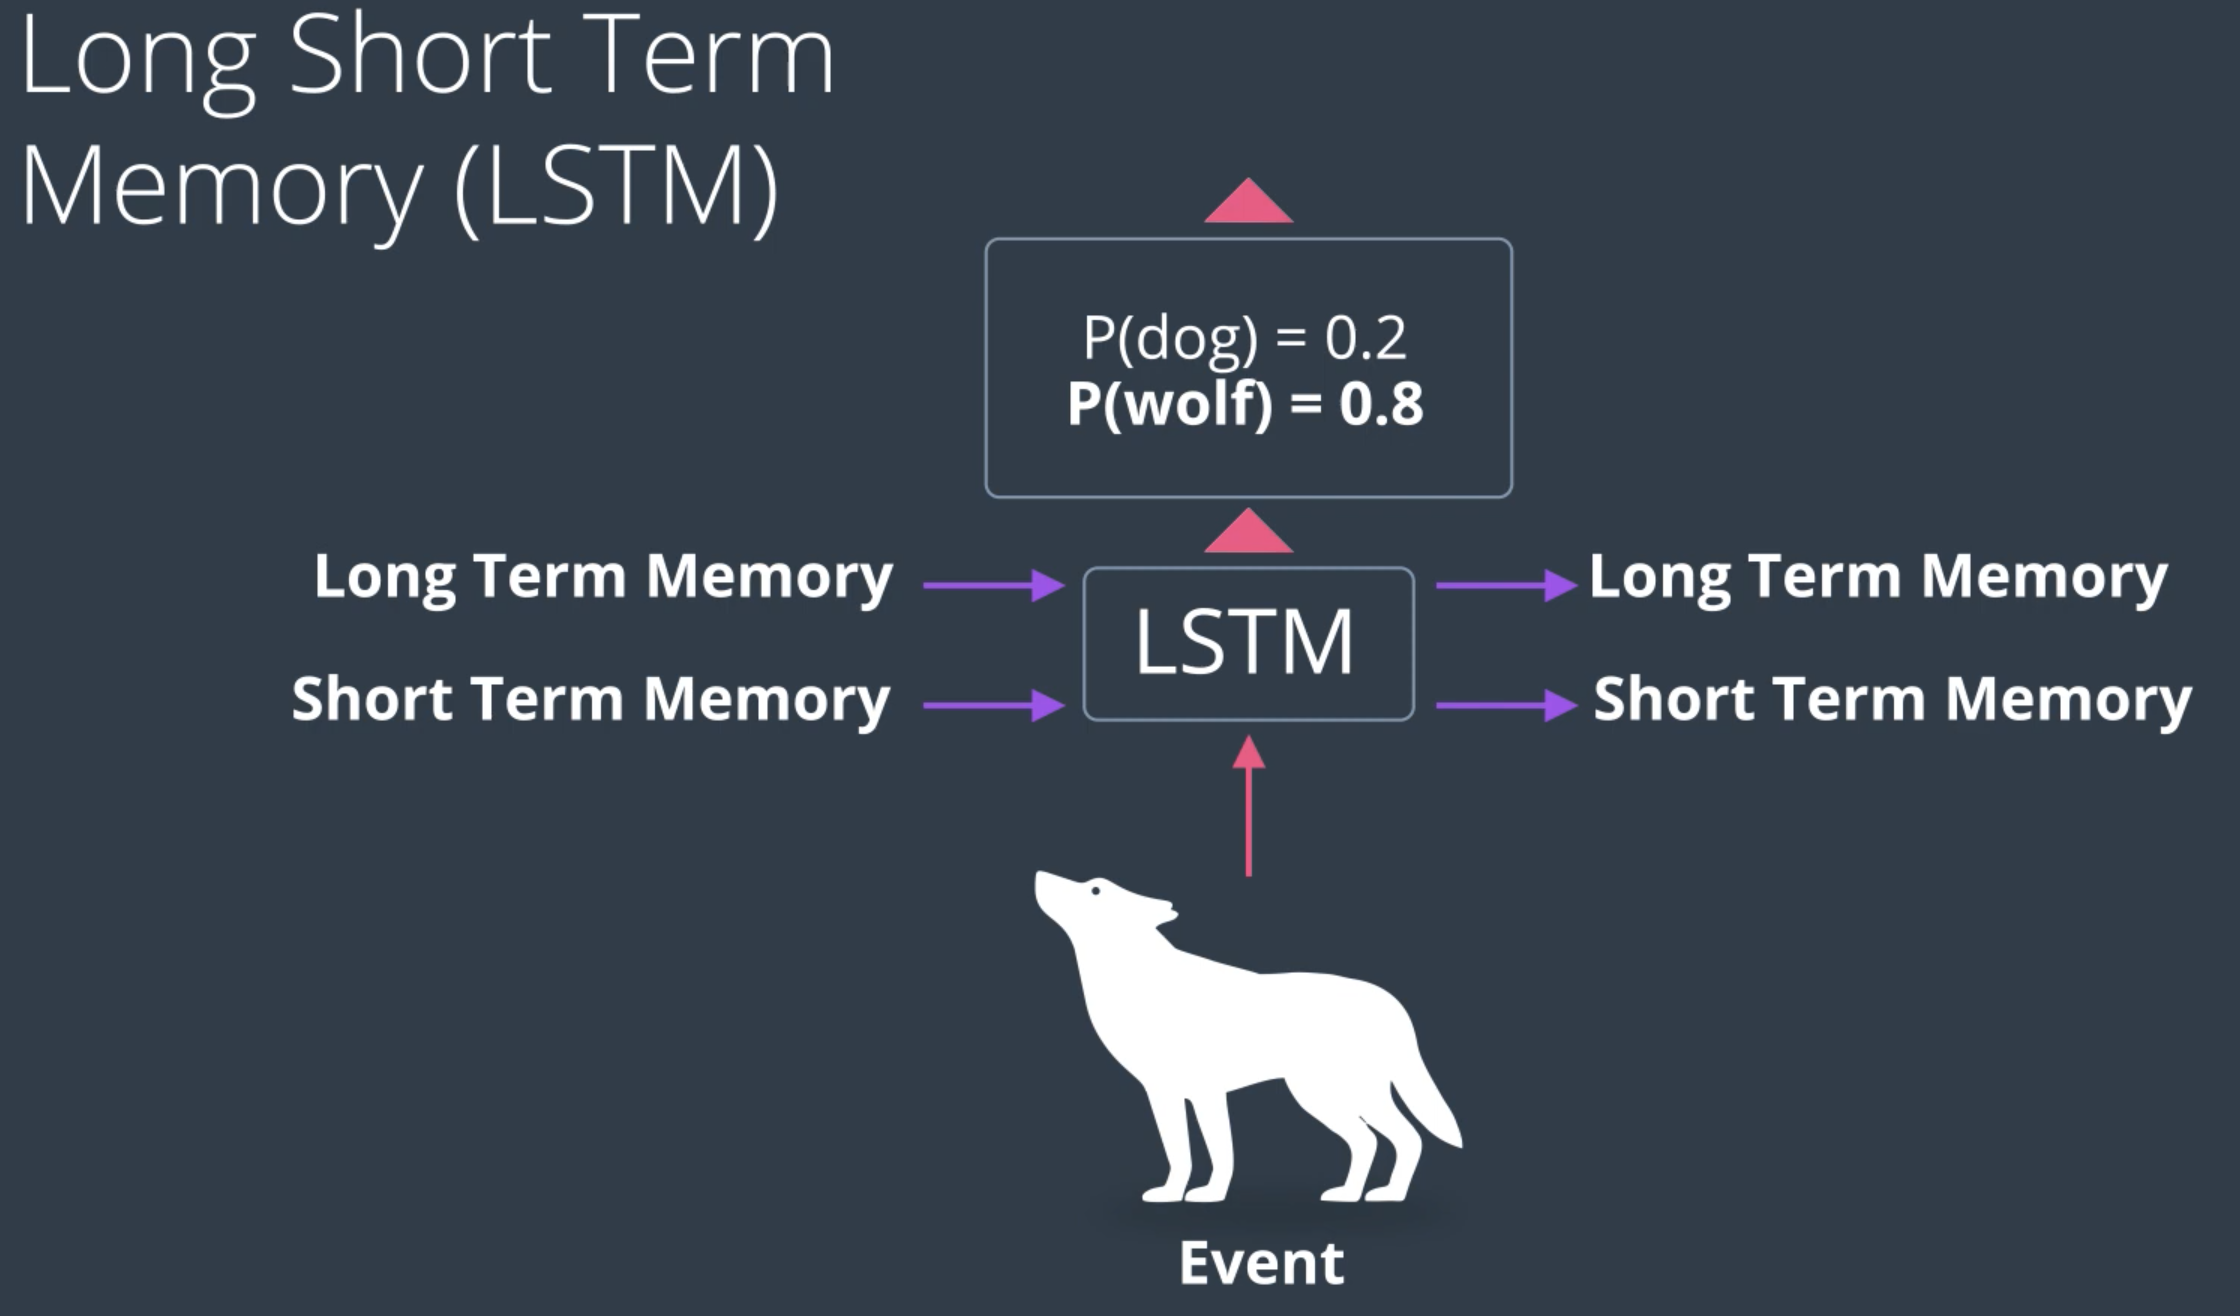
\includegraphics[width=1\linewidth]{img//rnn//lstm/longsthirttermmemory.png}

\section{From RNN to LSTM}

Before we take a close look at the \textbf{Long Short-Term Memory (LSTM)} cell, let's take a look at the following video: \href{https://www.youtube.com/watch?v=MsqybcWmzGY&ab_channel=Udacity}{Youtube} \newline

\textbf{Long Short-Term Memory Cells}, \href{http://www.bioinf.jku.at/publications/older/2604.pdf}{\textbf{(LSTM)}} give a solution to the vanishing gradient problem, by helping us apply networks that have temporal dependencies. They were proposed in 1997 by \href{https://en.wikipedia.org/wiki/Sepp_Hochreiter}{\textbf{Sepp Hochreiter}} and \href{http://people.idsia.ch/~juergen/}{\textbf{Jürgen Schmidhuber}} \newline

If we look closely at the RNN neuron, we see that we have simple linear combinations (with or without an activation function). We can also see that we have a single addition. \newline

Zooming in on the neuron, we can graphically see this in the following configuration:

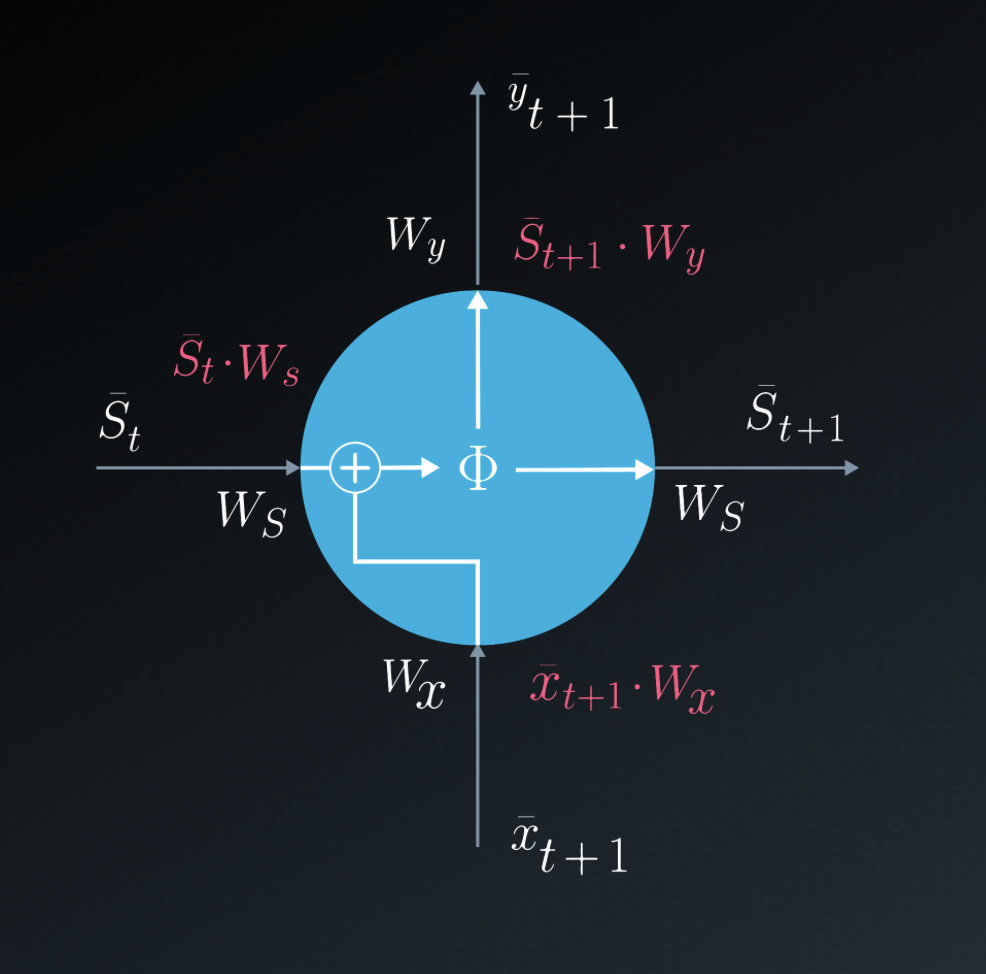
\includegraphics[width=0.5\linewidth]{img//rnn//lstm/screen-shot-2017-11-27-at-3.46.35-pm.png}
\captionof{figure}{Closeup Of The RNN Neuron}

\begin{itemize}
    \item Calculating the next stage: \(\overline{S}_{t+1} = \Phi (\overline{x}_{t+1} \cdot W_x + \overline{S}_t \cdot W_s)\)
    \item Calculating the output: \(\overline{y}_{t+1} = \overline{S}_{t+1} \cdot W_y\)
\end{itemize}

The \textbf{LSTM} cell is a bit more complicated. If we zoom in on the cell, we can see that the mathematical configuration is the following:

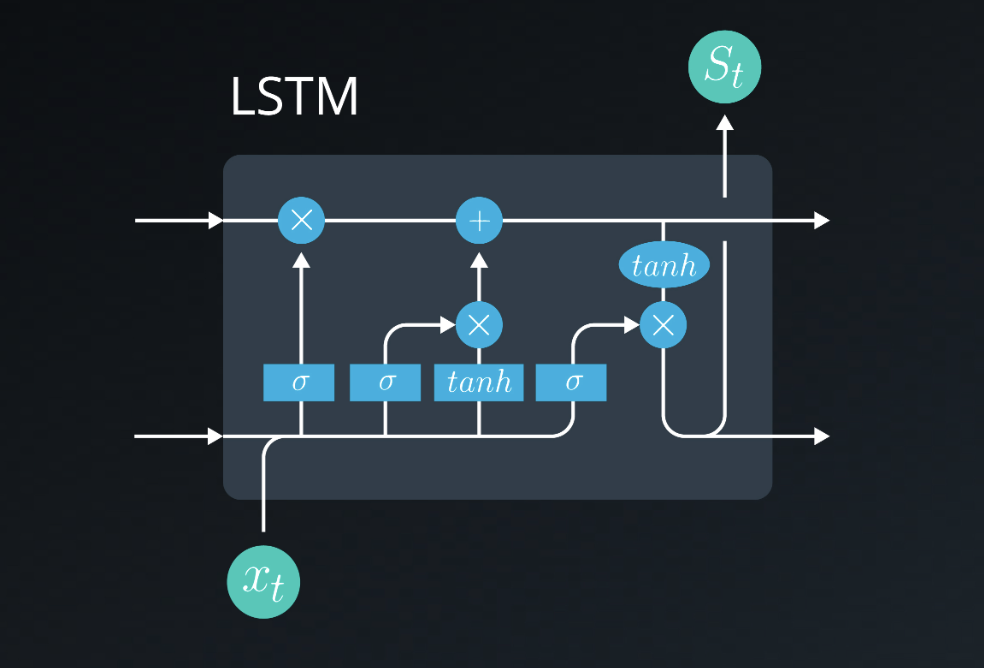
\includegraphics[width=0.5\linewidth]{img//rnn//lstm/screen-shot-2017-11-27-at-3.44.20-pm.png}
\captionof{figure}{Closeup Of the LSTM Cell}

Instead of a single calculation, we have 4 separate calculations:
\begin{enumerate}
    \item Sigma
    \item Hyperbolic tangent
    \item Multiplication
    \item Addition
\end{enumerate}

The LSTM cell allows a recurrent system to learn over many time steps without the fear of losing information due to the vanishing gradient problem. It is fully differentiable, therefore allowing us to use backpropagation when updating the weights easily. \newline

The main idea with LSTM cells is that they can decide which information to remove/forget, which information to store, and when to use it. The cell can also help decide when to move the previous state's information to the next. \newline

The LSTM cell has 3 sigmoids. The output of each sigmoid is between 0 and 1. This decides whether the data passes through or not.

\begin{itemize}
    \item All data passes through \(\sigma (x) \approx 1\)
    \item Data does not pass through: \(\sigma(x) \approx 0\)
\end{itemize}

Sigmoids act as a mechanism to filter
\begin{itemize}
    \item What goes into the cell, if at all
    \item What retains within the cell
    \item What passes to the output
\end{itemize}

\section{Basics of LSTM}
\href{https://www.youtube.com/watch?v=gjb68a4XsqE&t=5s&ab_channel=Udacity}{Youtube} \newline

In this video, we learned the basics of the LSTM. We have listed them below.

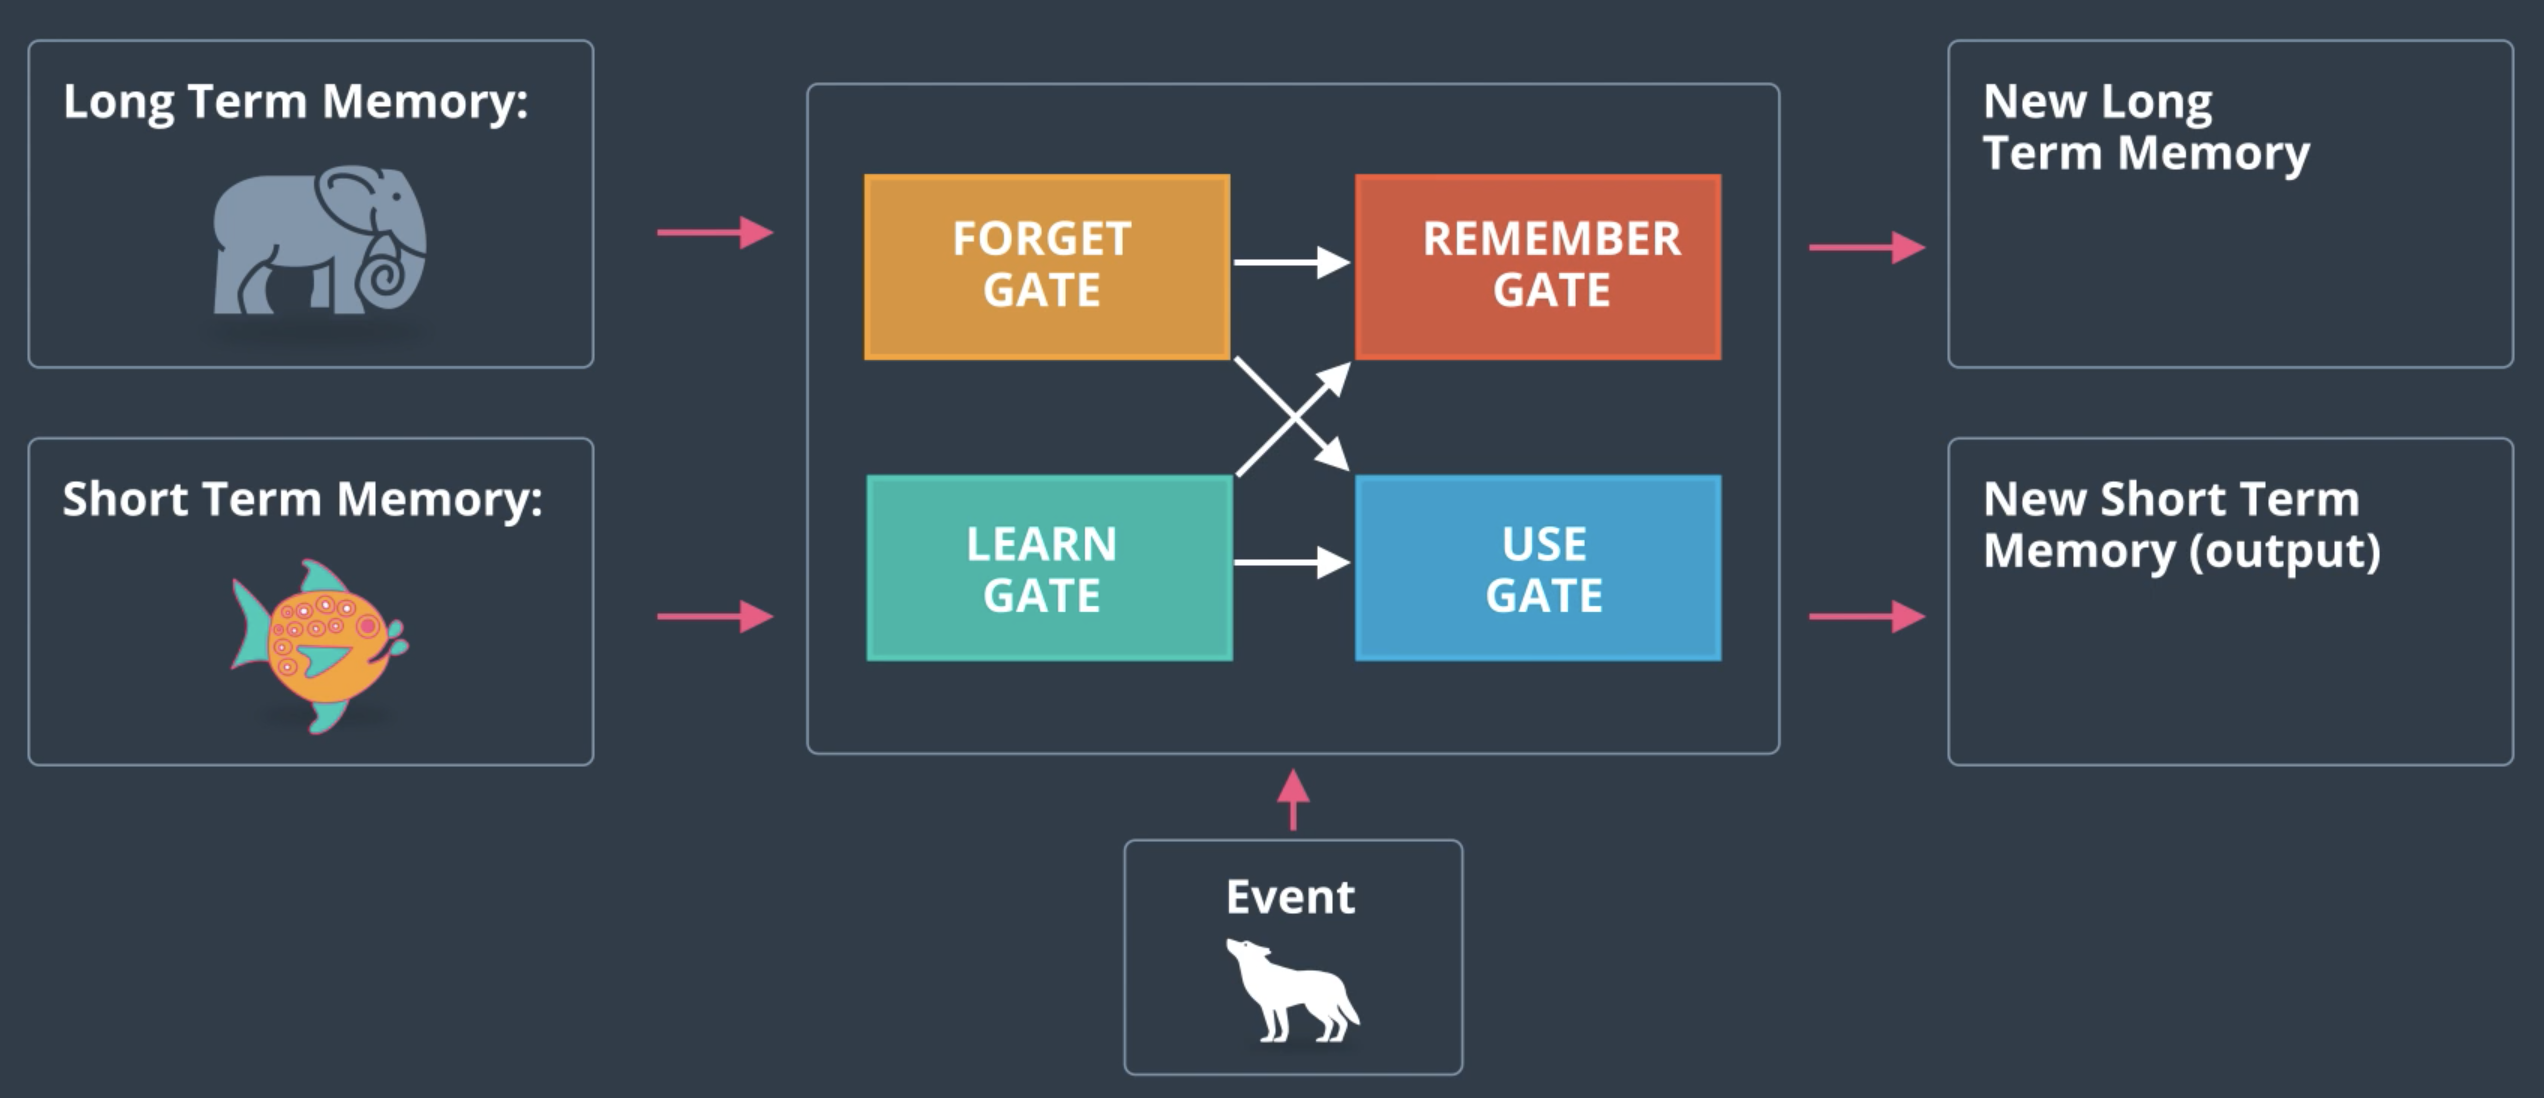
\includegraphics[width=1\linewidth]{img//rnn//lstm/basicsoflstm.png}

\textbf{Inputs}:
\begin{itemize}
    \item Long Term Memory
    \item Short Term Memory
    \item Input Vector (Event)
\end{itemize}

\textbf{Gates}:
\begin{itemize}
    \item Forget Gate
    \item Learn Gate
    \item Remember Gate
    \item Use Gate
\end{itemize}
\textbf{Outputs}:
\begin{itemize}
    \item New Long-Term Memory
    \item New Short-Term Memory
\end{itemize}

So the \textit{long term memory} goes to the forget gate where it forgets everything that it doesn't consider useful. The \textit{short term memory} and the \textit{event} are joined together in the \textit{learn gate}, containing the information that we've recently learned and it removes any unnecessary information.

Now the long term memory that we haven't forgotten yet plus the new information that we've learned get joined together in the \textit{remember gate}. This gate puts these two together and since it's called remember gate, what it does is it outputs an\textit{ updated long term memory}. So this is what we'll remember for the future.

And finally, the \textit{use gate} is the one that decides what information we use from what we previously know plus what we just learned to make a prediction so it also takes those inputs the long term memory,
and the new information joins them and decides what to output.
The \textit{output} becomes both the \textit{prediction} and the \textit{new short term memory}.

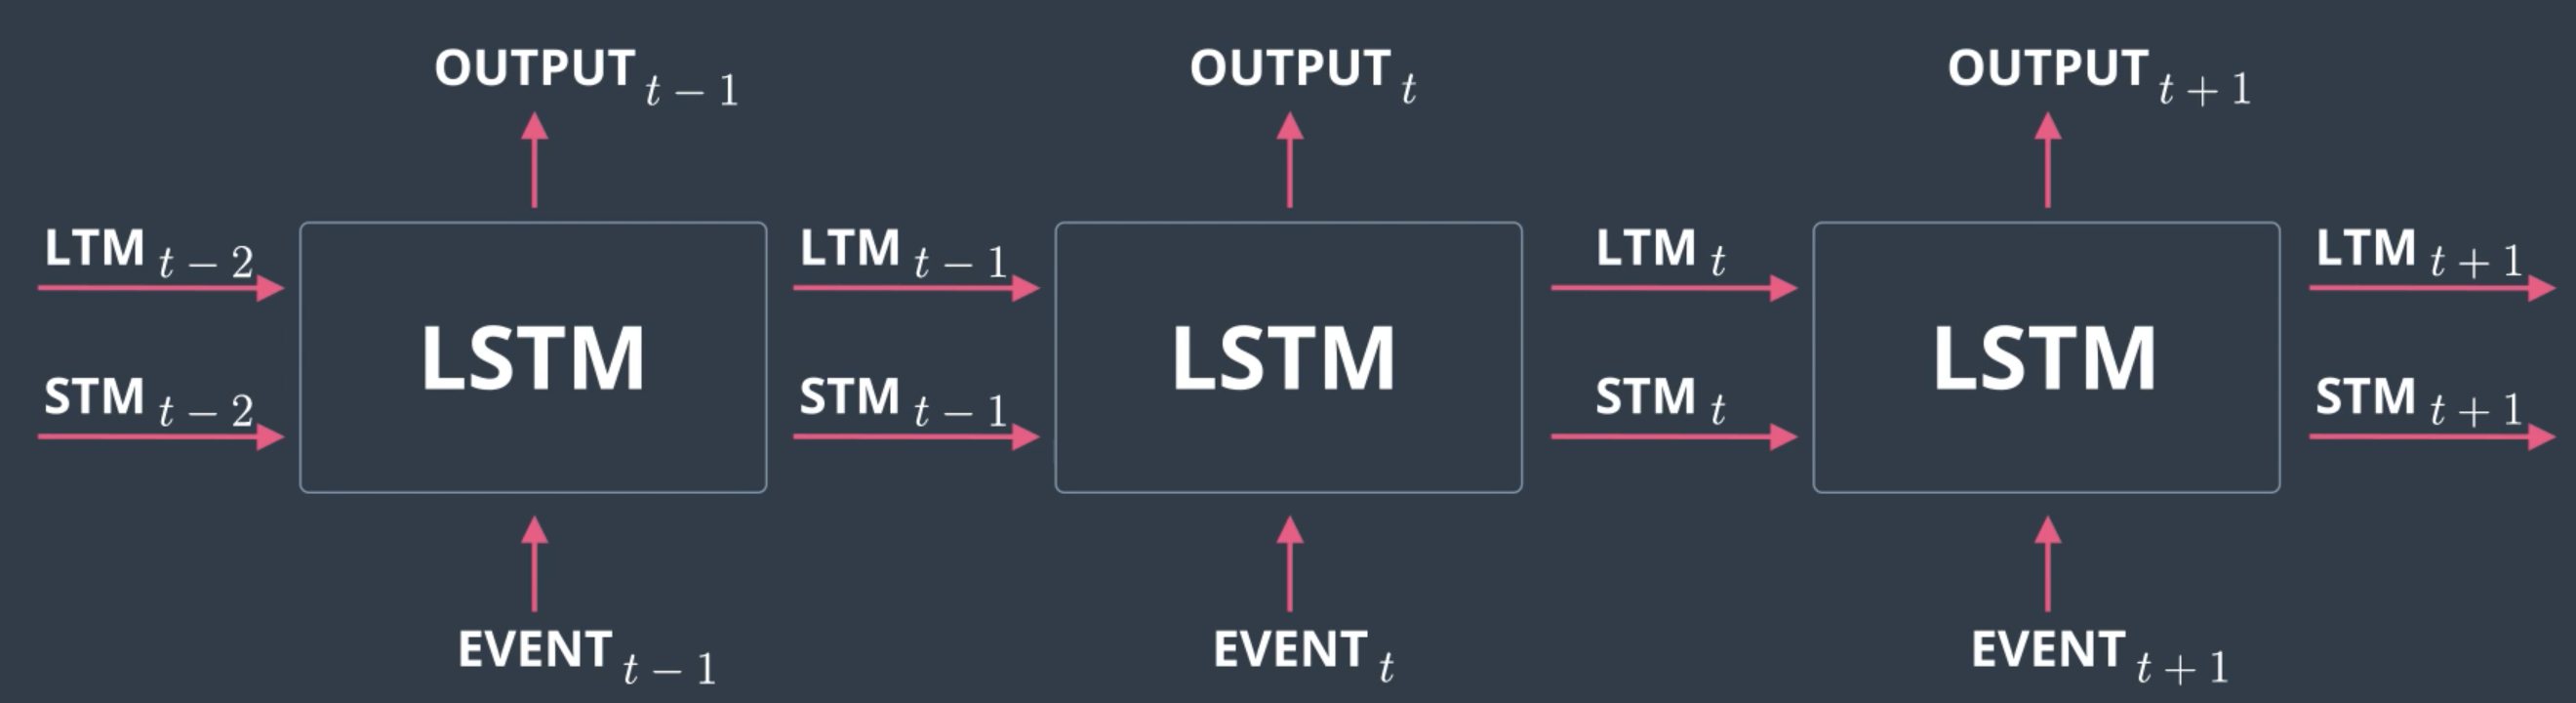
\includegraphics[width=1\linewidth]{img//rnn//lstm/basicsoflstm_general.png}


\section{Architecture of LSTM}
\href{https://www.youtube.com/watch?v=ycwthhdx8ws&t=4s&ab_channel=Udacity}{Youtube}

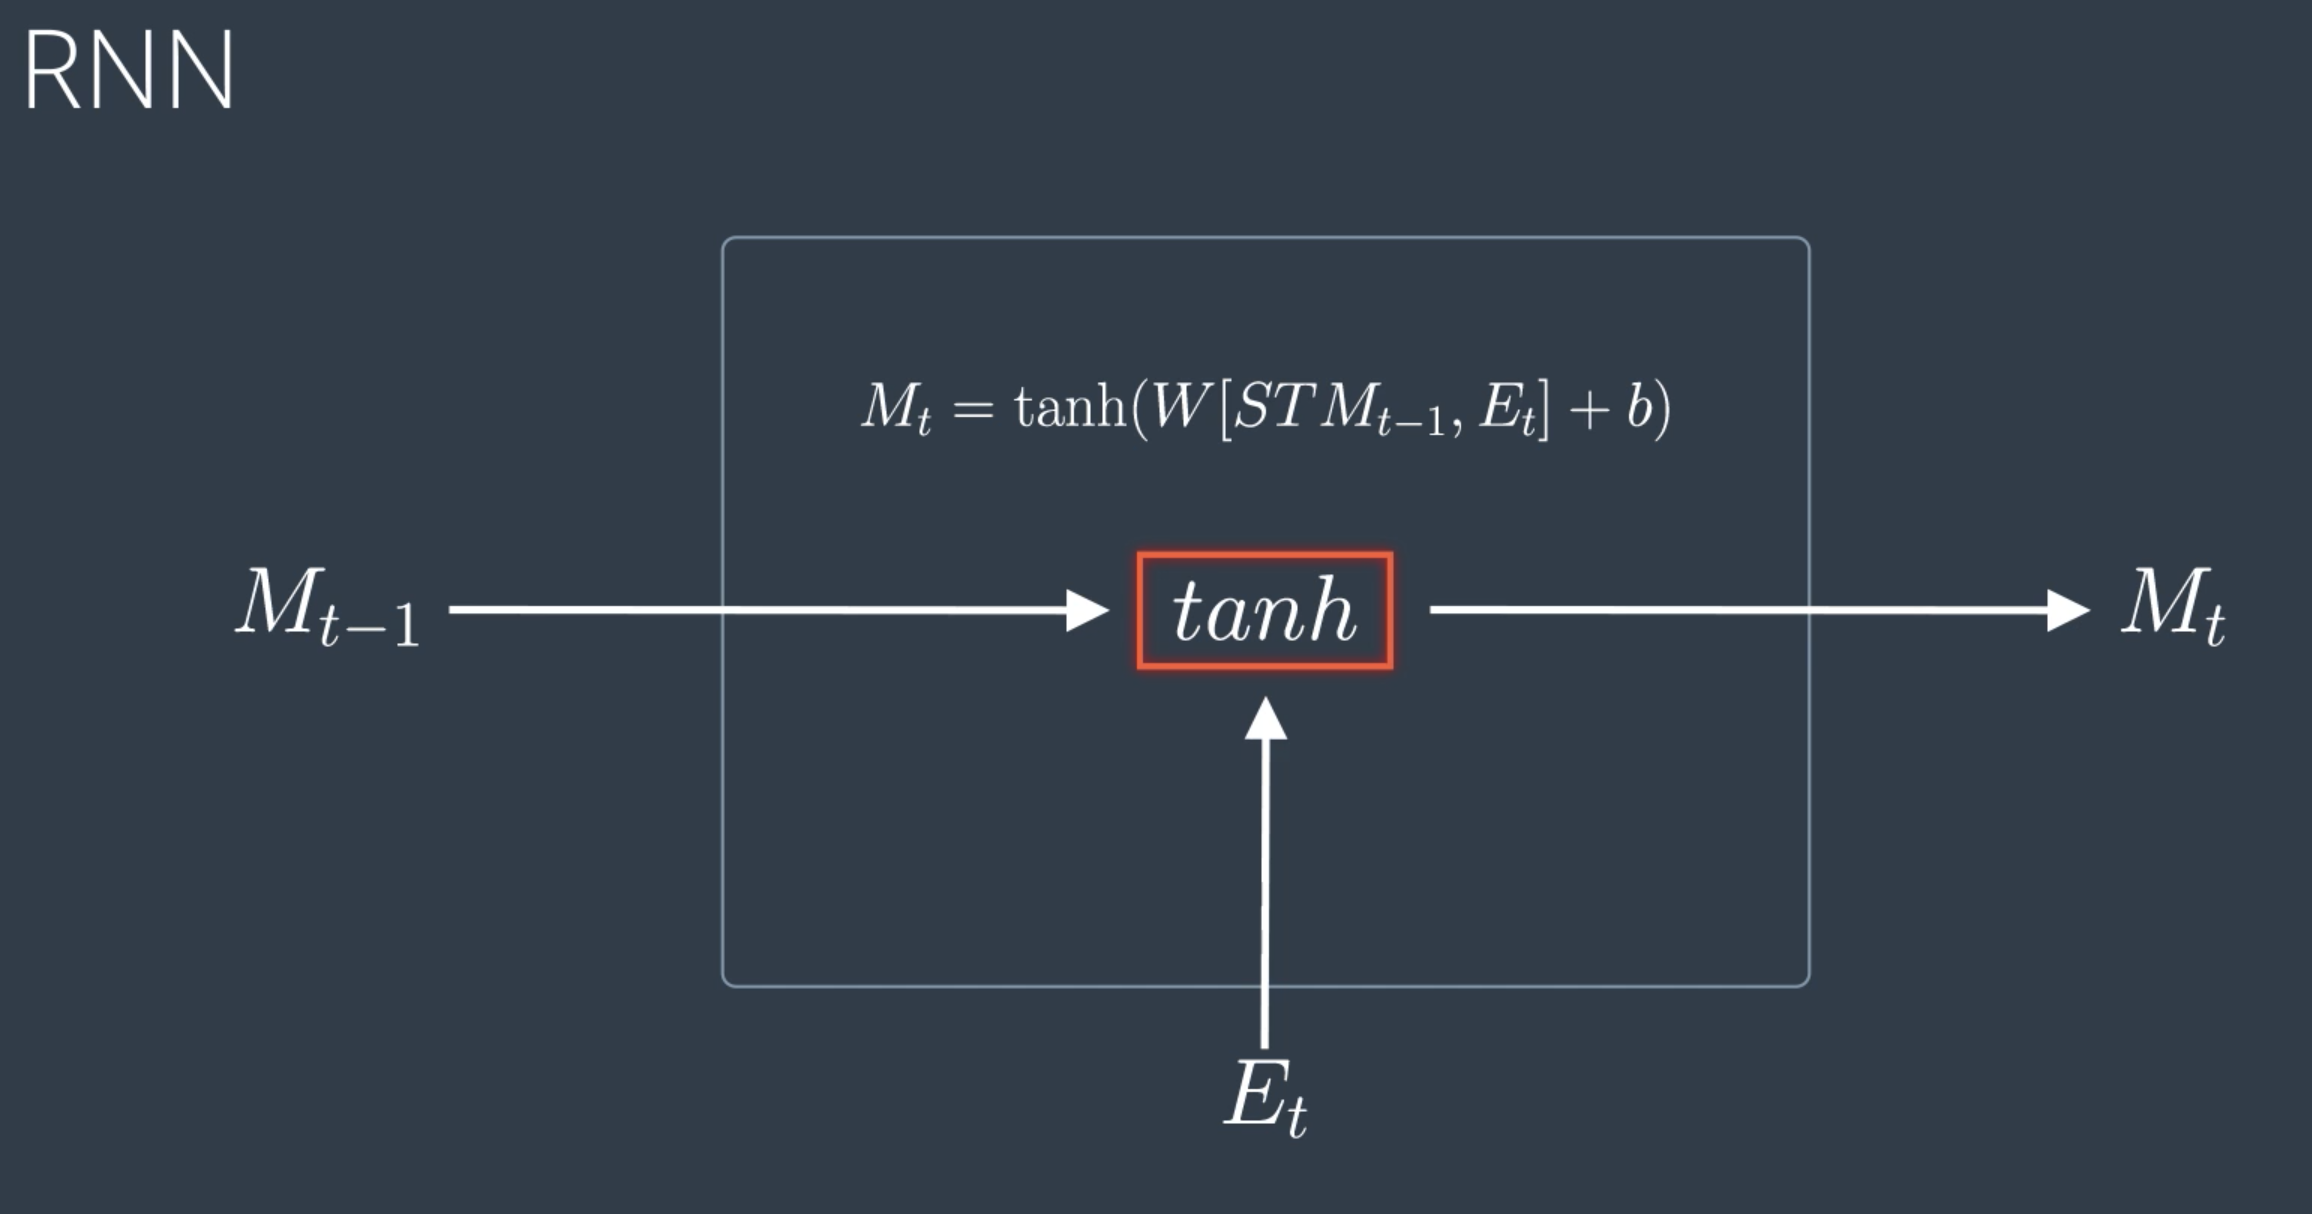
\includegraphics[width=1\linewidth]{img//rnn//lstm/rnnArchitecture.png}

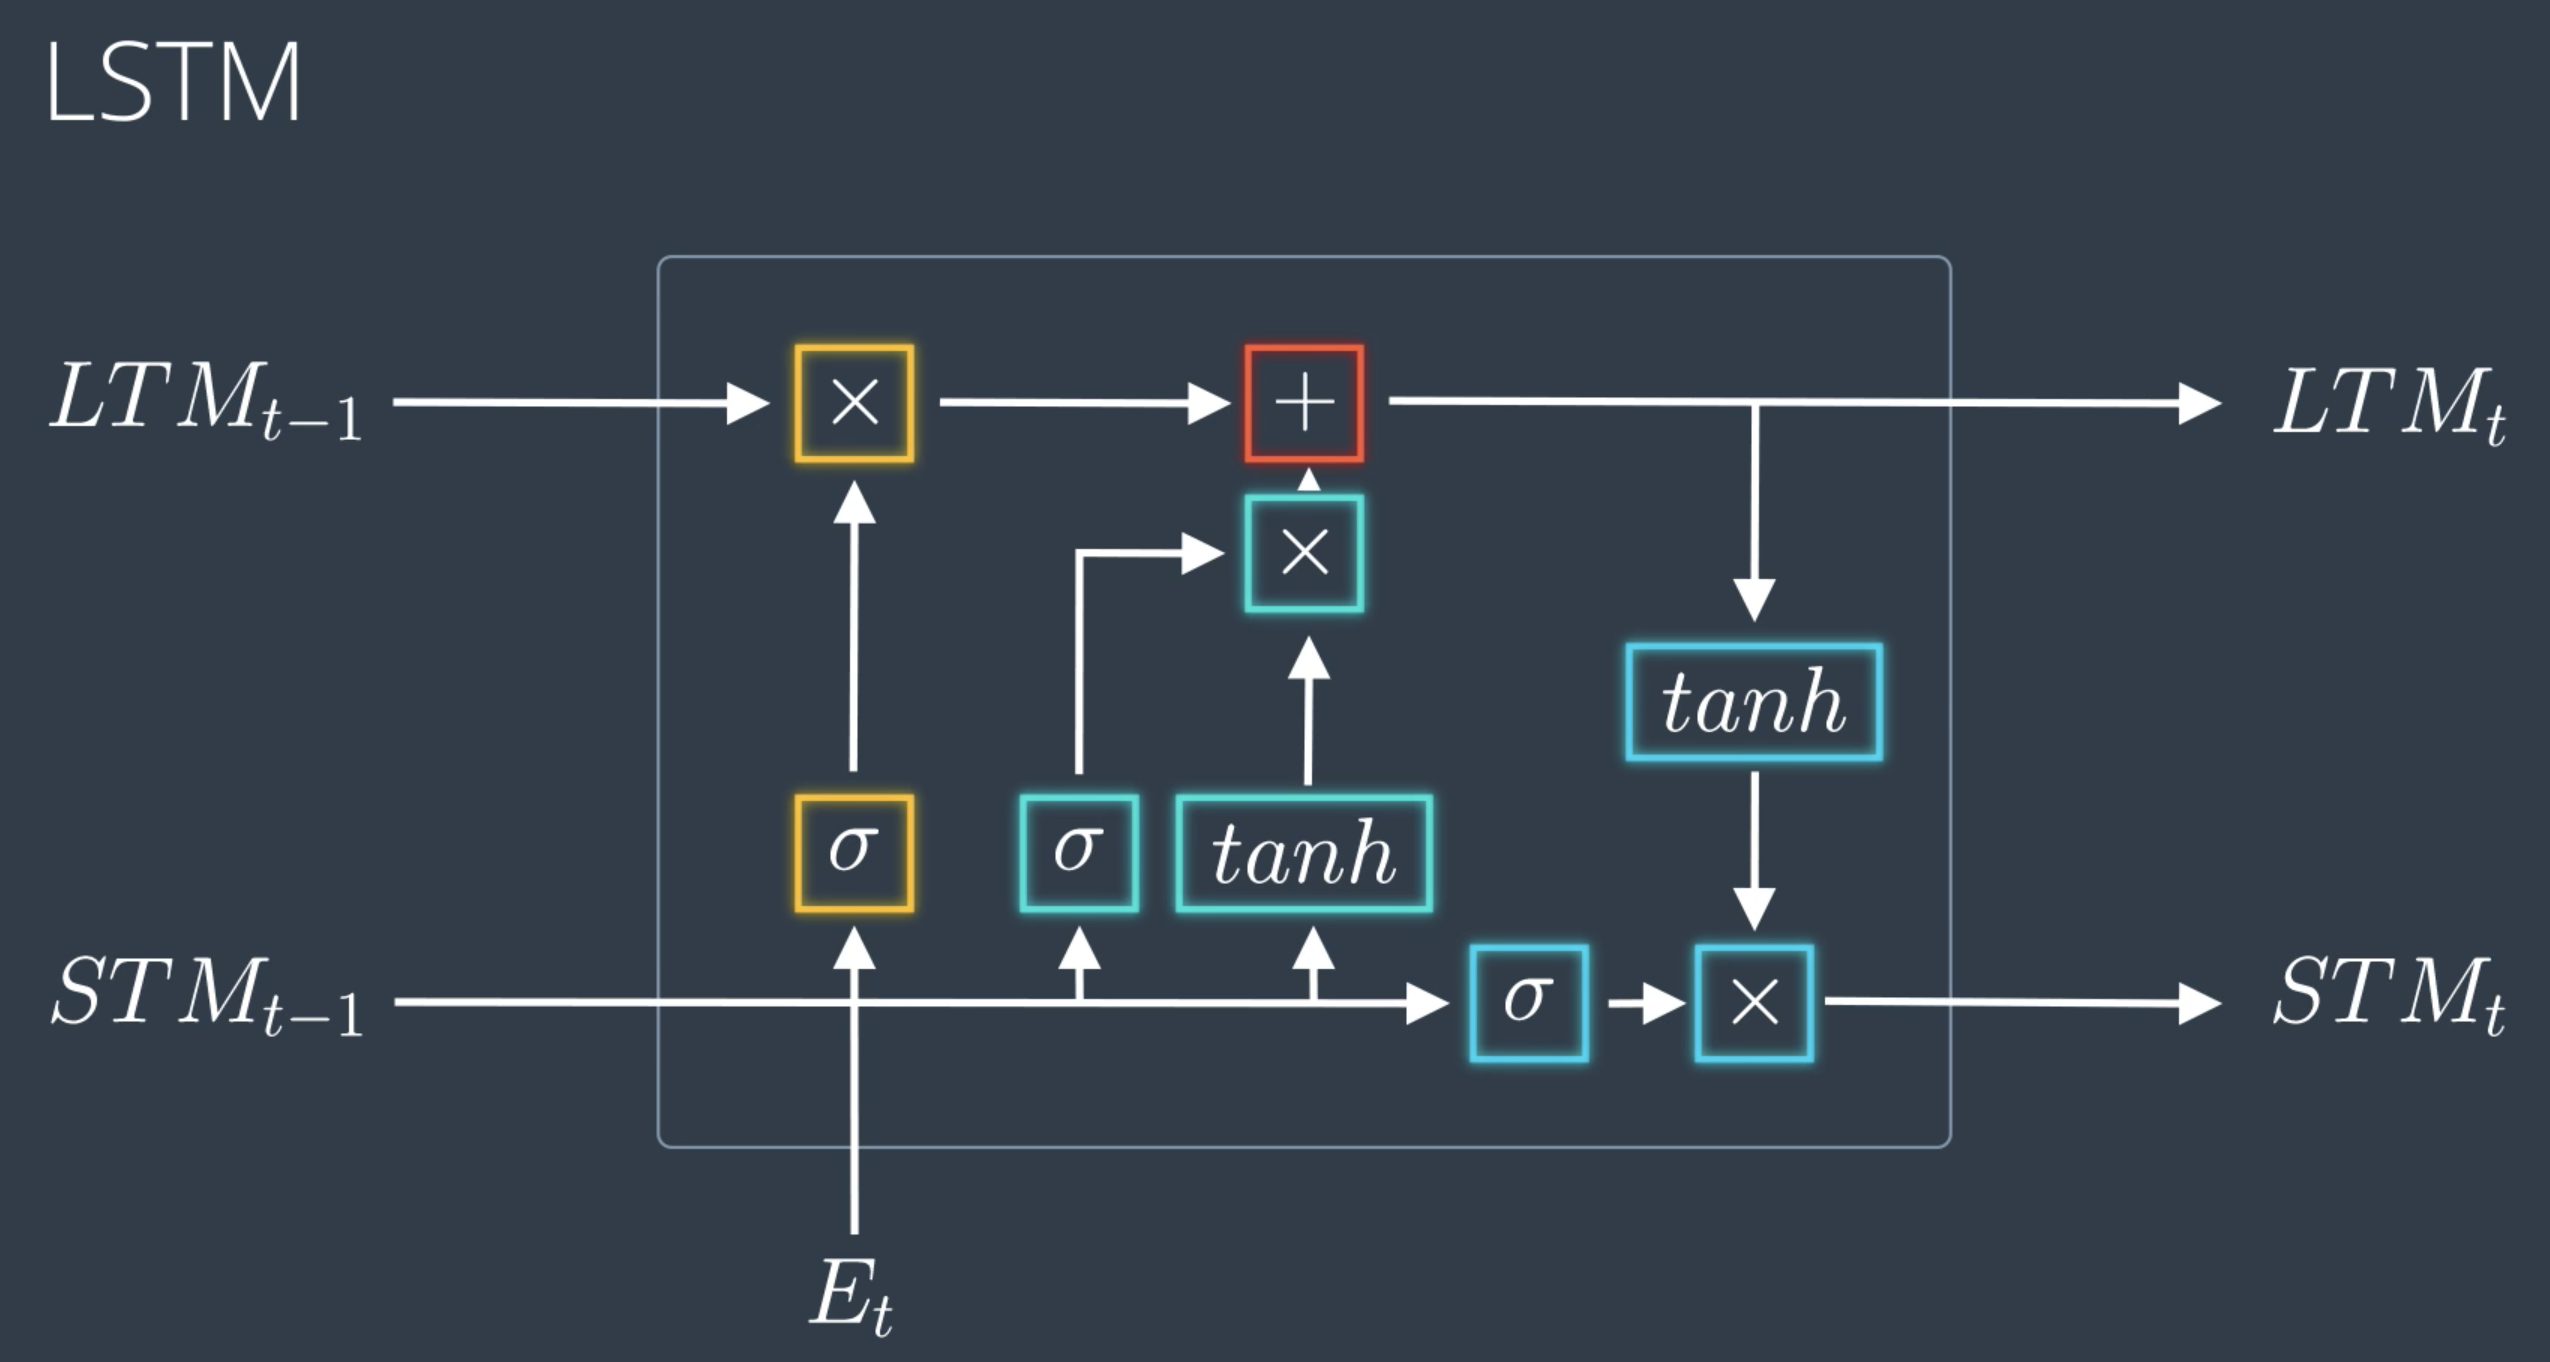
\includegraphics[width=1\linewidth]{img//rnn//lstm/lstmArchitecture.png}

\subsubsection{Quiz Question}

Check the important pieces of an LSTM architecture

The inputs of the input vector, LTM, and STM
\begin{itemize}
    \item \textbf{The inputs of the input vectors, LTM, and STM}
    \item The modulation factor
    \item \textbf{Forget, Learn, Remember, and Use Gates}
    \item The normalization gate
    \item \textbf{The Hidden State}
    \item \textbf{The outputs of the LTM and STM}
    \item \textbf{The Cell State}
\end{itemize}

\section{LSTM Gates}

\subsection{The Learn Gate}
\href{https://www.youtube.com/watch?v=aVHVI7ovbHY&t=2s&ab_channel=Udacity}{Youtube} \newline

The Learn Gate takes the short term memory (STM) and the event and joins them. Then it ignores a bit of it, keeping the important part. 

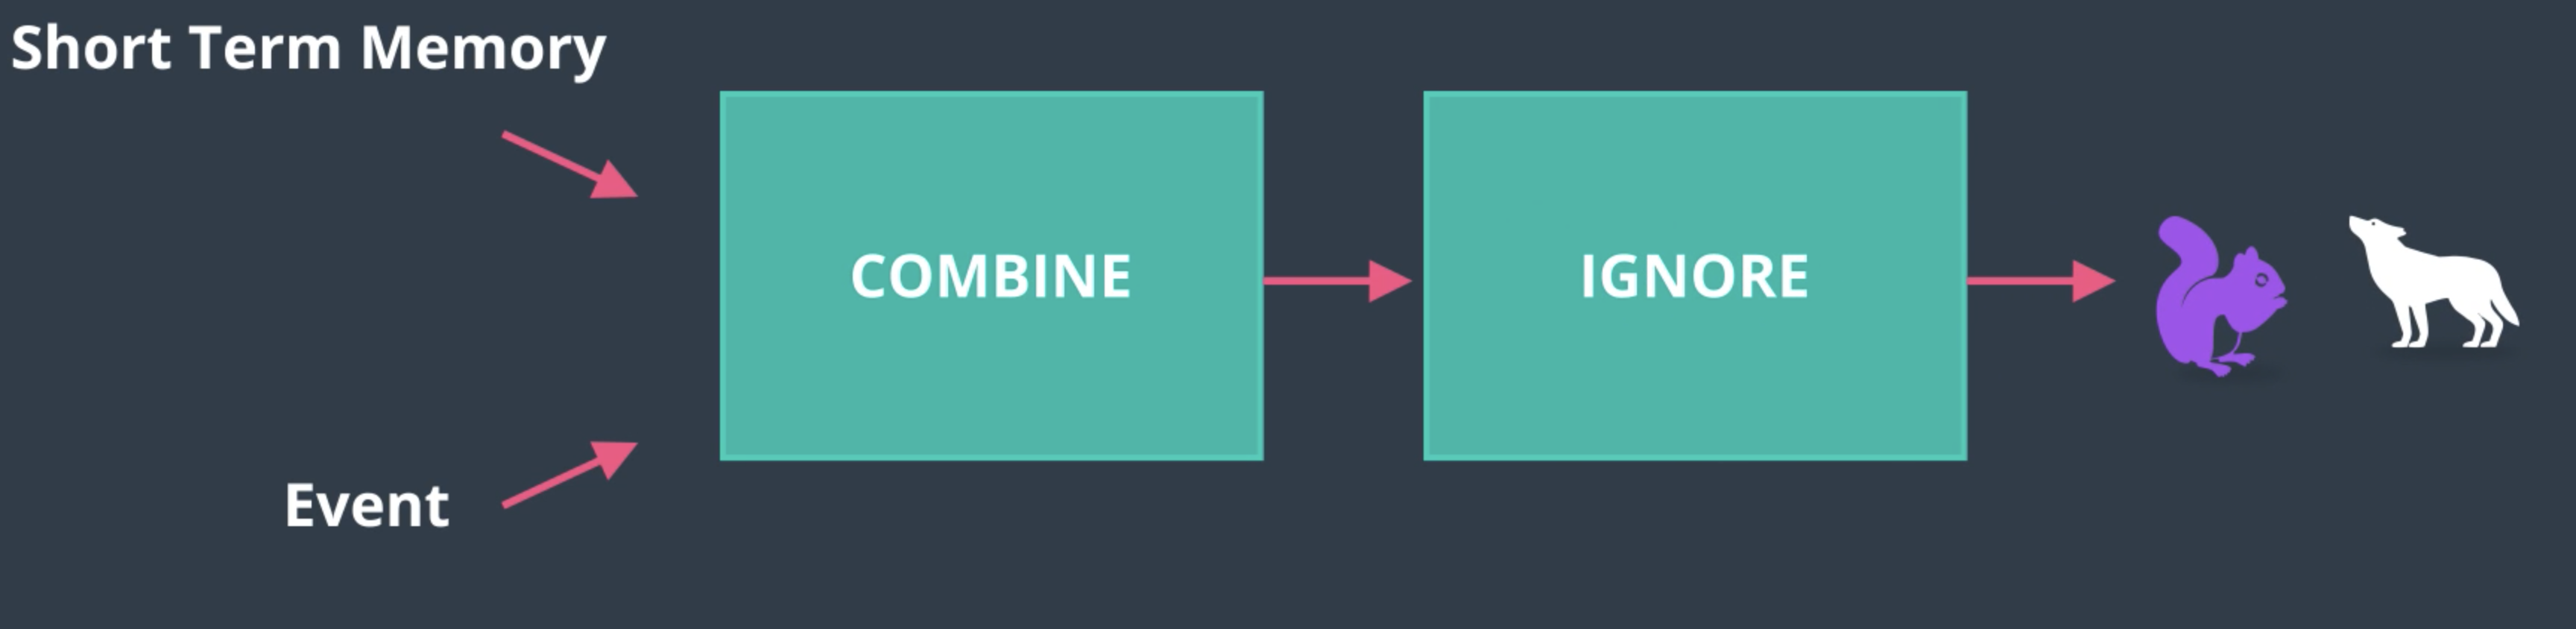
\includegraphics[width=1\linewidth]{img//rnn//lstm/learngate1.png}

The output of the \textit{Learn Gate} is \(N_t i_t\) where: 
\begin{equation} \label{eq:LearnGate}
\begin{split}
     N_t &= tanh(W_n [STM_{t-1}, E_t] + b_n) \\
    i_t &= \sigma(W_i [STM_{t-1}, E_t] + b_i)
\end{split}
\end{equation}
\begin{itemize}
    \item STM = Short term memory
    \item \(E_t\) = Event
    \item \(N_t\) = new information
\end{itemize}
In order to ignore part of the new information, we need to multiply the new information \(N_t\) with the ignore factor, \(i_t\), elementwise. 

\subsection{The Forget Gate}
\href{https://www.youtube.com/watch?v=iWxpfxLUPSU&ab_channel=Udacity}{Youtube} \newline

The output of the \textit{Forget Gate} is \(LTM_{t-1} f_t\) where:
\begin{equation}\label{eq:forgetGate}
    f_t = \sigma(W_f[STM_{t-1}, E_t] + b_f)
\end{equation}
\begin{itemize}
    \item LTM = Long Term Memory
    \item \(f_t\) = Forget factor
\end{itemize}

\subsection{The Remember Gate}
\href{https://www.youtube.com/watch?v=0qlm86HaXuU&ab_channel=Udacity}{Youtube} \newline

The \textit{remember gate} takes the LTM coming out of the \textit{forget gate} and the STM coming out of the \textit{learn gate} and simply combines them together. 

The output of the \textit{Remember Gate} is:
\begin{equation}
    LTM_{t-1} f_t + N_t i_t
\end{equation}
(\(N_t\), \(i_t\), and \(f_t\) are calculated in \autoref{eq:LearnGate} and \autoref{eq:forgetGate})


\subsection{The Use Gate}
\href{https://www.youtube.com/watch?v=IFBXQBfnS5g&ab_channel=Udacity}{Youtube} \newline

The output of the \textit{Use Gate} is \(U_t V_t\) where:
\begin{equation}
    \begin{split}
        U_t &= tanh(W_u LTM_{t-1} f_t + b_u) \\
        V_t &= \sigma(W_v [STM_{t-1}, E_t] + b_v)
    \end{split}
\end{equation}
The output is \(STM_t = U_t \cdot V_t\)

\subsection{Quiz Question}

Match each LSTM gate to it's function.

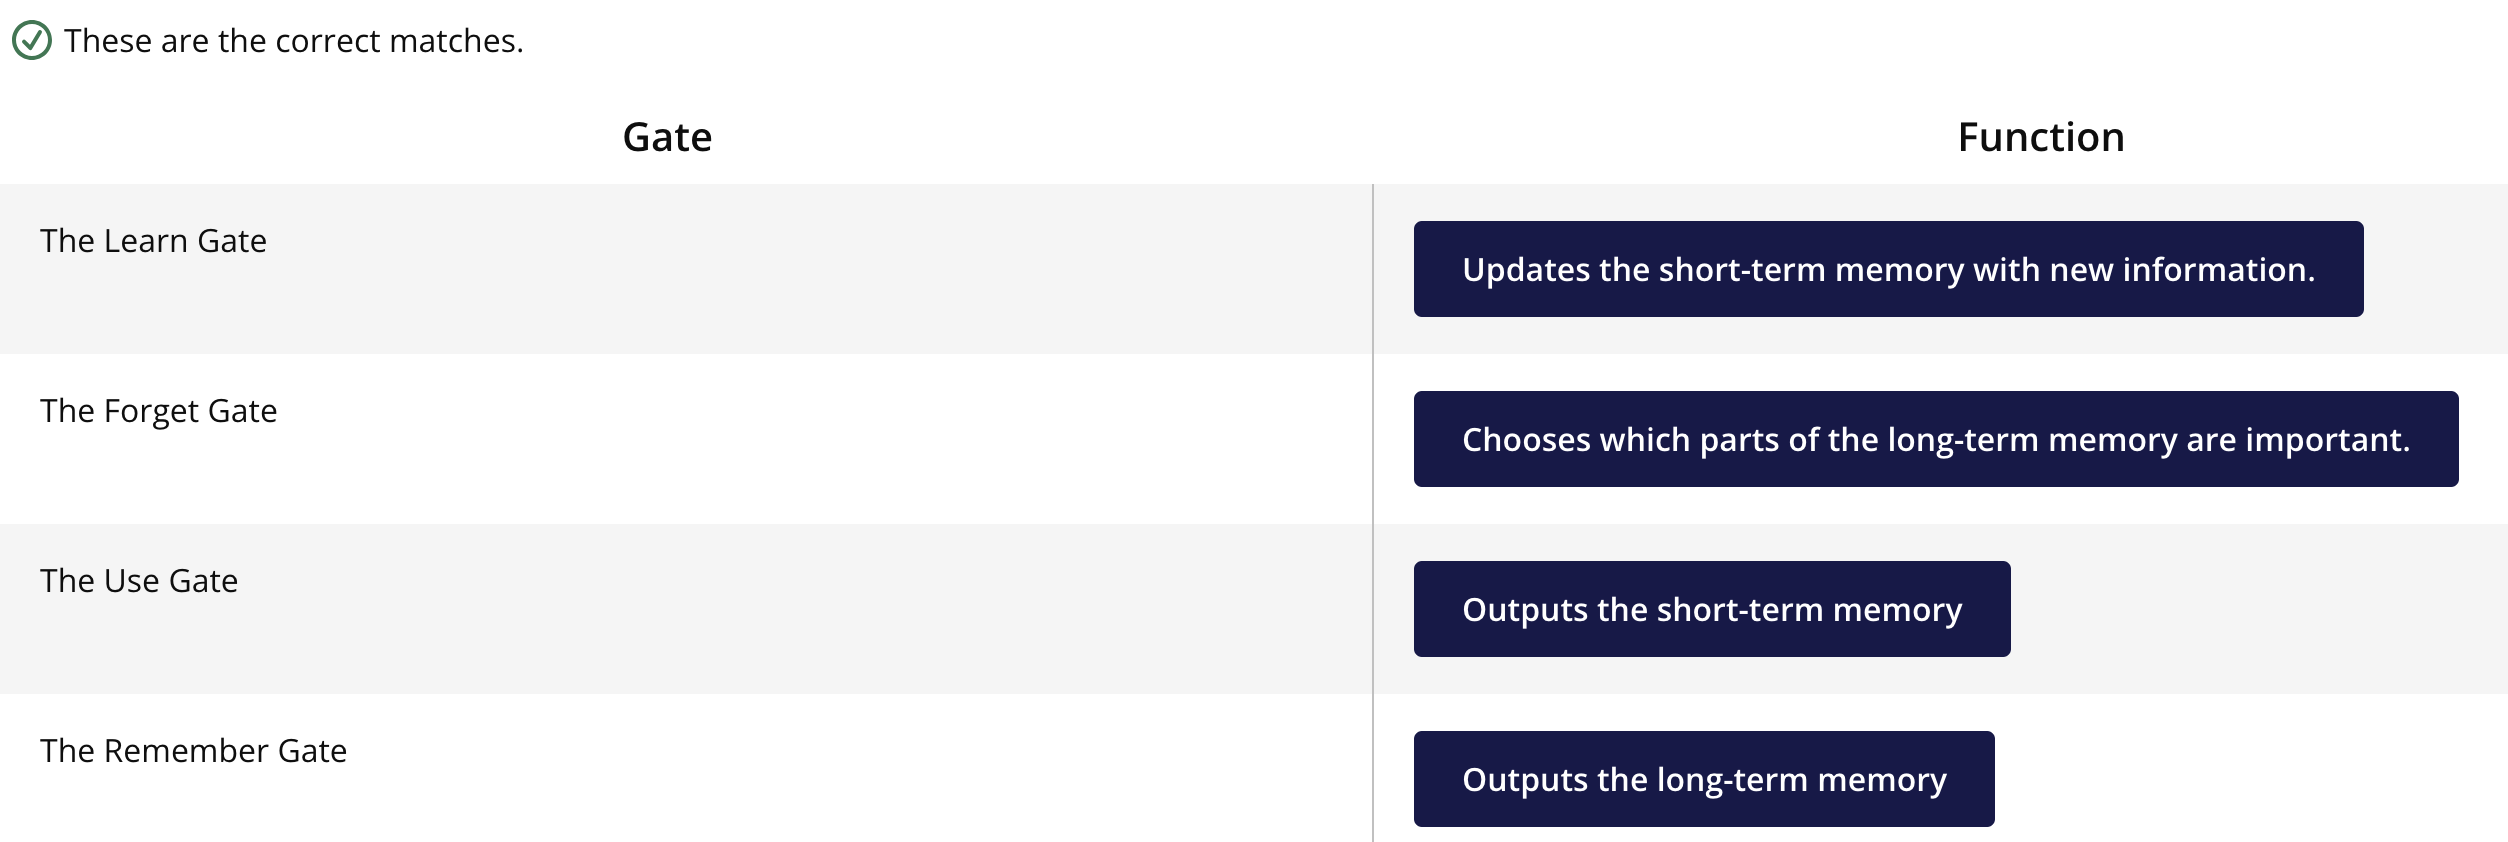
\includegraphics[width=1\linewidth]{img//rnn//lstm/gates_quiz.png}

\subsection{Putting it together}
\href{https://www.youtube.com/watch?v=IF8FlKW-Zo0&ab_channel=Udacity}{Youtube}

\section{Quiz}
If you would like to deepen your knowledge even more, go over the following \href{https://web.archive.org/web/20190106151528/https://skymind.ai/wiki/lstm}{\textbf{tutorial}}. Focus on the overview titled: \textbf{Long Short-Term Memory Units (LSTMs)}. \newline

If you are feeling confident enough, skip the overview and jump right into our next question:

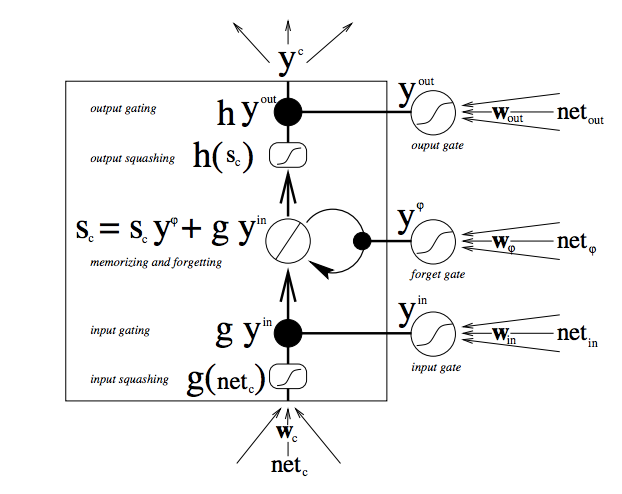
\includegraphics[width=0.5\linewidth]{img//rnn//lstm/screen-shot-2017-11-16-at-5.54.40-pm.png}
\captionof{figure}{The LSTM cell- taken form the Deep Learning tutorial}


\subsubsection{Quiz Question}

The illustration above is of a LSTM cell. What would be the values of the three gates in situations where the cell retains information for a long period, without accepting a new input or producing an output?

\begin{itemize}
    \item \textbf{The inputs gate: close to 0; the forget gate: close to 1; the output gate: close to 0}
    \item The inputs gate: close to 1; the forget gate: close to 1; the output gate: close to 0
    \item The inputs gate: close to 0; the forget gate: close to 0; the output gate: close to 0
    \item The inputs gate: close to 0; the forget gate: close to 1; the output gate: close to 1
\end{itemize}

\section{Predicting Temperature Time Series with LSTM Using
PyTorch}\label{predicting-temperature-time-series-with-lstm-using-pytorch}

\subsubsection{Introduction}\label{introduction}

Long Short-Term Memory (LSTM) is a type of recurrent neural network
(RNN) that is commonly used for sequence modeling, particularly for
processing time-series data. Unlike traditional RNNs, LSTMs have a
memory cell that allows them to selectively remember or forget
information over time, which makes them particularly useful for
long-term dependencies.

In this tutorial, we'll use Pytorch to build an LSTM model that can
predict a time-series based on previous data. We'll use numpy and pandas
to preprocess the data.

\subsection{Step 1: Import Libraries}\label{step-1-import-libraries}

We'll start by importing the necessary libraries.

\begin{lstlisting}[language=Python]
import numpy as np
import pandas as pd
import torch
import torch.nn as nn
\end{lstlisting}

\begin{lstlisting}
/opt/venv/lib/python3.10/site-packages/tqdm/auto.py:21: TqdmWarning: IProgress not found. Please update jupyter and ipywidgets. See https://ipywidgets.readthedocs.io/en/stable/user_install.html
  from .autonotebook import tqdm as notebook_tqdm
\end{lstlisting}

\subsubsection{Step 2: Load Data}\label{step-2-load-data}

For this tutorial, we'll use a sample dataset that contains temperature
readings for a single sensor over time. We'll load the dataset into a
pandas DataFrame and preprocess it so that it can be fed into our LSTM
model.

\begin{lstlisting}[language=Python]
# Load data into a pandas DataFrame
df = pd.read_csv('../data/temperature.csv')

# Convert the 'datetime' column to a datetime object
df['Date'] = pd.to_datetime(df['Date'])

# Set the 'datetime' column as the index
df.set_index('Date', inplace=True)

# Resample the data to hourly intervals and fill missing values with the previous value
df = df.resample('H').ffill()

# Normalize the data
df = (df - df.mean()) / df.std()

# Convert the DataFrame to a numpy array
data = df.values
\end{lstlisting}

\subsubsection{Step 3: Split Data}\label{step-3-split-data}

Next, we'll split the data into training and testing sets. We'll use the
first 70\% of the data for training and the remaining 30\% for testing.

\begin{lstlisting}[language=Python]
# Split the data into training and testing sets
train_size = int(len(data) * 0.7)
train_data, test_data = data[:train_size], data[train_size:]
\end{lstlisting}

\subsubsection{Step 4: Create Data
Sequences}\label{step-4-create-data-sequences}

Before we can train our LSTM model, we need to create sequences of data
that the model can learn from. We'll create sequences of length 24 (one
day), and we'll use a sliding window approach to create overlapping
sequences.

\begin{lstlisting}[language=Python]
# Function to create sequences of data
def create_sequences(data, seq_length):
    X = []
    y = []
    for i in range(len(data) - seq_length):
        X.append(data[i:i+seq_length])
        y.append(data[i+seq_length])
    return np.array(X), np.array(y)

# Create sequences for training and testing data
seq_length = 24
X_train, y_train = create_sequences(train_data, seq_length)
X_test, y_test = create_sequences(test_data, seq_length)
\end{lstlisting}

\subsubsection{Step 5: Create LSTM
Model}\label{step-5-create-lstm-model}

Now, we'll create our LSTM model using Pytorch. Our model will have one
LSTM layer with 32 hidden units and one fully connected output layer.

\begin{lstlisting}[language=Python]
class LSTM(nn.Module):
    def __init__(self, input_size, hidden_size, output_size):
        super(LSTM, self).__init__()
        self.lstm = nn.LSTM(input_size, hidden_size, batch_first=True)
        self.fc = nn.Linear(hidden_size, output_size)

    def forward(self, x):
        out, _ = self.lstm(x)
        out = self.fc(out[:, -1, :])
        return out
\end{lstlisting}

In the \lstinline{\_\_init\_\_} method, we define an LSTM
layer with hidden\_size hidden units and a fully connected output layer
with output\_size output units. In the forward method, we pass the input
\lstinline{x} through the LSTM layer, take the output of
the last time step, and pass it through the fully connected output
layer.

\subsubsection{Step 6: Instantiate Model and Define Loss Function and
Optimizer}\label{step-6-instantiate-model-and-define-loss-function-and-optimizer}

Now, we'll instantiate our LSTM model, define our loss function (mean
squared error), and define our optimizer (Adam).

\begin{lstlisting}[language=Python]
# Instantiate the model
input_size = X_train.shape[2]
hidden_size = 32
output_size = 1
model = LSTM(input_size, hidden_size, output_size)

# Define the loss function and optimizer
criterion = nn.MSELoss()
optimizer = torch.optim.Adam(model.parameters(), lr=0.001)
\end{lstlisting}

\subsubsection{Step 7: Train the Model}\label{step-7-train-the-model}

Next, we'll train our LSTM model on the training data. We'll use a batch
size of 32 and train for 50 epochs.

\begin{lstlisting}[language=Python]
# Convert numpy arrays to Pytorch tensors
X_train = torch.from_numpy(X_train).float()
y_train = torch.from_numpy(y_train).float()
X_test = torch.from_numpy(X_test).float()
y_test = torch.from_numpy(y_test).float()

# Define the batch size and number of epochs
batch_size = 32
num_epochs = 25

# Train the model
for epoch in range(num_epochs):
    # Shuffle the training data
    perm = torch.randperm(X_train.shape[0])
    X_train = X_train[perm]
    y_train = y_train[perm]

    # Loop over batches
    for i in range(0, X_train.shape[0], batch_size):
        # Get batch
        batch_X = X_train[i:i+batch_size]
        batch_y = y_train[i:i+batch_size]

        # Zero the gradients
        optimizer.zero_grad()

        # Forward pass
        outputs = model(batch_X)
        loss = criterion(outputs, batch_y)

        # Backward pass and optimization
        loss.backward()
        optimizer.step()

    # Print loss for this epoch
    print('Epoch [{}/{}], Loss: {:.4f}'.format(epoch+1, num_epochs, loss.item()))
\end{lstlisting}

\begin{lstlisting}
Epoch [1/25], Loss: 3.4126
Epoch [2/25], Loss: 0.0009
Epoch [3/25], Loss: 0.0003
Epoch [4/25], Loss: 0.0001
Epoch [5/25], Loss: 0.0001
Epoch [6/25], Loss: 0.0010
Epoch [7/25], Loss: 0.0367
Epoch [8/25], Loss: 0.0002
Epoch [9/25], Loss: 0.1150
Epoch [10/25], Loss: 0.0002
Epoch [11/25], Loss: 0.0001
Epoch [12/25], Loss: 0.0003
Epoch [13/25], Loss: 0.0000
Epoch [14/25], Loss: 0.0000
Epoch [15/25], Loss: 0.0001
Epoch [16/25], Loss: 0.0013
Epoch [17/25], Loss: 0.0000
Epoch [18/25], Loss: 0.0006
Epoch [19/25], Loss: 0.0000
Epoch [20/25], Loss: 0.0000
Epoch [21/25], Loss: 0.0000
Epoch [22/25], Loss: 0.0009
Epoch [23/25], Loss: 0.0005
Epoch [24/25], Loss: 0.0000
Epoch [25/25], Loss: 0.0000
\end{lstlisting}

\subsubsection{Step 8: Evaluate the
Model}\label{step-8-evaluate-the-model}

Finally, we'll evaluate our LSTM model on the testing data.

\begin{lstlisting}[language=Python]
# Evaluate the model on the test data
model.eval()
with torch.no_grad():
    y_pred = model(X_test)

# Calculate the test loss
test_loss = criterion(y_pred, y_test)
print('Test Loss: {:.4f}'.format(test_loss.item()))
\end{lstlisting}

\begin{lstlisting}
Test Loss: 0.0167
\end{lstlisting}

\begin{lstlisting}[language=Python]
import matplotlib.pyplot as plt

# Convert Pytorch tensors to numpy arrays
y_test = y_test.numpy()
y_pred = y_pred.numpy()

# Plot predicted vs actual values
plt.figure(figsize=(10, 6))
plt.plot(y_test[:500], label='Actual')
plt.plot(y_pred[:500], label='Predicted')
plt.xlabel('Time Step')
plt.ylabel('Value')
plt.title('LSTM Predictions')
plt.legend()
plt.show()
\end{lstlisting}

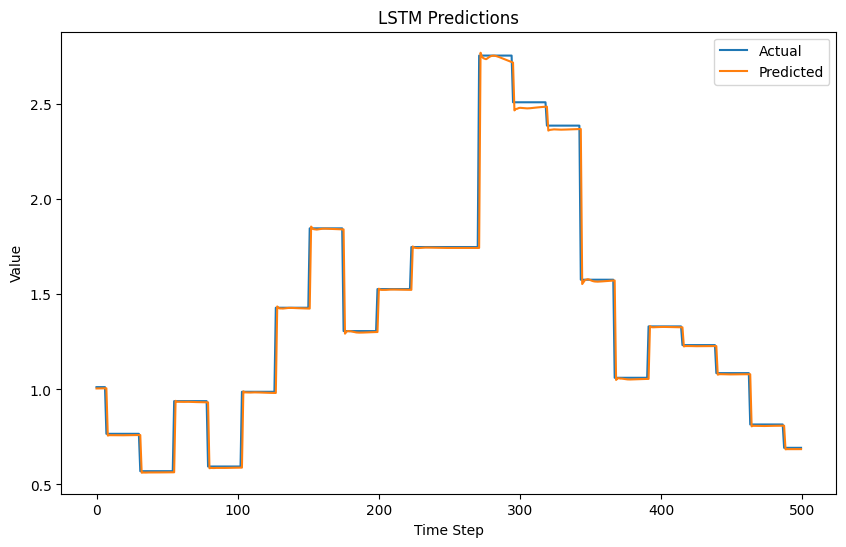
\includegraphics{img/rnn/lstm/output_16_0_pred_temp.png}


\section{Sentiment Analysis using
LSTM}\label{sentiment-analysis-using-lstm}

\begin{lstlisting}[language=Python]
import torch
import torch.nn as nn
import torch.optim as optim
\end{lstlisting}

\begin{lstlisting}
/opt/venv/lib/python3.10/site-packages/tqdm/auto.py:21: TqdmWarning: IProgress not found. Please update jupyter and ipywidgets. See https://ipywidgets.readthedocs.io/en/stable/user_install.html
  from .autonotebook import tqdm as notebook_tqdm
\end{lstlisting}

\paragraph{Prepare data}\label{prepare-data}

\begin{lstlisting}[language=Python]
# Sentences (textual data) and their sentiment labels (1 for positive, 0 for negative)
sentences = ["i love this movie", "this film is amazing", "i didn't like it", "it was terrible"]
sentiment = [1, 1, 0, 0]
\end{lstlisting}

\paragraph{Create Vocabulary}\label{create-vocabulary}

\begin{lstlisting}[language=Python]
# Simple vocabulary to represent words as indices
vocab = {"<PAD>": 0, "i": 1, "love": 2, "this": 3, "movie": 4, "film": 5, "is": 6, "amazing": 7, "didn't": 8, "like": 9, "it": 10, "was": 11, "terrible": 12}
\end{lstlisting}

We create a simple vocabulary to represent words as indices. This allows
us to convert words in our sentences to numbers, which can be fed as
input to our neural network.

\paragraph{Tokenize, encode and pad
sentences}\label{tokenize-encode-and-pad-sentences}

\begin{lstlisting}[language=Python]
encoded_sentences = [[vocab[word] for word in sentence.split()] for sentence in sentences]
max_length = max([len(sentence) for sentence in encoded_sentences])
padded_sentences = [sentence + [vocab["<PAD>"]] * (max_length - len(sentence)) for sentence in encoded_sentences]
\end{lstlisting}

We tokenize and encode the sentences using the vocabulary created
earlier. We also pad the sentences with the
\lstinline{<PAD>} token to make them all the same length.

\paragraph{Convert data to tensors}\label{convert-data-to-tensors}

\begin{lstlisting}[language=Python]
inputs = torch.LongTensor(padded_sentences)
labels = torch.FloatTensor(sentiment)
\end{lstlisting}

We convert the input data and labels to PyTorch tensors. Inputs are
converted to LongTensors, while labels are converted to FloatTensors.

\paragraph{Define LSTM Model}\label{define-lstm-model}

\begin{lstlisting}[language=Python]
class SimpleLSTM(nn.Module):
    def __init__(self, vocab_size, embedding_dim, hidden_dim, output_dim):
        super(SimpleLSTM, self).__init__()
        self.embedding = nn.Embedding(vocab_size, embedding_dim)
        self.lstm = nn.LSTM(embedding_dim, hidden_dim)
        self.fc = nn.Linear(hidden_dim, output_dim)

    def forward(self, x):
        embedded = self.embedding(x)
        output, (hidden, _) = self.lstm(embedded)
        logits = self.fc(hidden.squeeze(0))
        return logits
\end{lstlisting}

We define a simple LSTM model class that inherits from
\lstinline{nn.Module}. The model consists of an embedding
layer, an LSTM layer, and a fully connected (linear) layer. The forward
method takes an input tensor \lstinline{x}, passes it
through the embedding layer, the LSTM layer, and finally the fully
connected layer to produce the output logits.

\paragraph{Instantiate model and define loss and
optimizer}\label{instantiate-model-and-define-loss-and-optimizer}

\begin{lstlisting}[language=Python]
model = SimpleLSTM(len(vocab), embedding_dim=10, hidden_dim=20, output_dim=1)
criterion = nn.BCEWithLogitsLoss()
optimizer = optim.Adam(model.parameters(), lr=0.001)
\end{lstlisting}

We instantiate the LSTM model with the vocabulary size, embedding
dimensions, hidden dimensions, and output dimensions. We also define the
binary cross-entropy with logits loss
(\lstinline{BCEWithLogitsLoss}) and the Adam optimizer.

\paragraph{Train the model}\label{train-the-model}

\begin{lstlisting}[language=Python]
epochs = 1000
for epoch in range(epochs):
    optimizer.zero_grad()
    predictions = model(inputs.t()).squeeze(1)
    loss = criterion(predictions, labels)
    loss.backward()
    optimizer.step()

    if (epoch + 1) % 100 == 0:
        print(f"Epoch: {epoch + 1}, Loss: {loss.item()}")
\end{lstlisting}

\begin{lstlisting}
Epoch: 100, Loss: 0.15219397842884064
Epoch: 200, Loss: 0.02454642578959465
Epoch: 300, Loss: 0.010403754189610481
Epoch: 400, Loss: 0.006161490920931101
Epoch: 500, Loss: 0.004242383409291506
Epoch: 600, Loss: 0.0031633577309548855
Epoch: 700, Loss: 0.002477444475516677
Epoch: 800, Loss: 0.0020062942057847977
Epoch: 900, Loss: 0.0016651706537231803
Epoch: 1000, Loss: 0.001408295938745141
\end{lstlisting}

We train the model for 1000 epochs. In each epoch, we:

\begin{itemize}
\item Reset the gradients by calling optimizer.zero\_grad()
\item Get the model's predictions for the input sentences by calling model(inputs.t()).squeeze(1)
\item Calculate the loss between the predictions and the true labels using the criterion defined earlier
\item Perform backpropagation by calling loss.backward()
\item Update the model's parameters by calling optimizer.step()
\item We also print the loss every 100 epochs for monitoring the training progress.
\end{itemize}

\paragraph{Test the model}\label{test-the-model}

\begin{lstlisting}[language=Python]
with torch.no_grad():
    test_sentences = ["i love this film", "it was terrible"]
    encoded_test_sentences = [[vocab[word] for word in sentence.split()] for sentence in test_sentences]
    padded_test_sentences = [sentence + [vocab["<PAD>"]] * (max_length - len(sentence)) for sentence in encoded_test_sentences]
    test_inputs = torch.LongTensor(padded_test_sentences)
    test_predictions = torch.sigmoid(model(test_inputs.t()).squeeze(1))
    print("Test predictions:", test_predictions)
\end{lstlisting}

\begin{lstlisting}
Test predictions: tensor([0.9958, 0.0011])
\end{lstlisting}

We test the model on two new sentences. First, we tokenize, encode, and
pad the test sentences in the same way as we did for the training
sentences. We then convert the test sentences to PyTorch tensors and
pass them through the model. We apply the sigmoid function to the output
logits to obtain the final predictions, which represent the probability
of each sentence being positive.

The resulting \lstinline{test\_predictions} tensor
contains the model's sentiment predictions for the given test sentences.

